\documentclass[a4paper,twocolumn,11pt,nopdfoutputerror]{quantumarticle}
\usepackage[utf8]{inputenc}
\usepackage[T1]{fontenc}
\usepackage[english]{babel}
\usepackage{amsmath,amssymb,amsthm,mathtools}
\usepackage{braket}
\usepackage{graphicx}
\usepackage{booktabs}
\usepackage{siunitx}
\usepackage{microtype}
\usepackage{xcolor}
\usepackage[numbers,sort&compress]{natbib}
\usepackage[ruled,vlined]{algorithm2e}
\usepackage{enumitem}
\usepackage{multirow}
\usepackage{bbm}
\usepackage{makecell}

% ---------- macros ----------
\DeclareMathOperator{\Tr}{Tr}
\newcommand{\F}{\mathbb{F}}
\newcommand{\R}{\mathbb{R}}
\newcommand{\Pauli}{\mathcal{P}}
\newcommand{\synd}{\mathbf{s}}
\newcommand{\err}{\mathbf{e}}
\newcommand{\ehat}{\hat{\mathbf{e}}}
\newcommand{\llr}{\Lambda}
\newcommand{\Hmat}{\mathbf{H}}
\newcommand{\Gmat}{\mathbf{G}}
\newcommand{\Wmat}{\mathbf{W}}
\newcommand{\bvec}[1]{\mathbf{#1}}
\newcommand{\phat}{\hat{p}}
\newcommand{\concat}{\,\|\,}
\newcommand{\code}[3]{\ensuremath{[\![#1,#2,#3]\!]}}
\newcommand{\pending}[1]{\textcolor{red}{\textbf{[#1]}}}
\newtheorem{proposition}{Proposition}
\newtheorem{remark}{Remark}

\graphicspath{{./figures/}{./}}
\DeclareGraphicsExtensions{.pdf,.png,.jpg}

\usepackage{hyperref}
\hypersetup{colorlinks=true,citecolor=blue,linkcolor=blue,urlcolor=blue}

% ============================================================
%  TITLE
% ============================================================
\title{GNN-Augmented BP Architectures for QLDPC Decoding}

\author{Jothiradithya Sai Konduru}
\affiliation{Paradise Valley High School, Phoenix, AZ, USA}

\author{Anish Chedalla}
\affiliation{Paradise Valley High School, Phoenix, AZ, USA}

\author{Nithin Raveendran}
\affiliation{Department of Electrical and Computer Engineering,
             University of Arizona, Tucson, AZ, USA}
\email{nithin@arizona.edu}


\begin{document}
\maketitle

% ============================================================
%  ABSTRACT
% ============================================================
\begin{abstract}
Bivariate bicycle (BB) quantum low-density parity-check (QLDPC) codes
combine finite encoding rate with low-weight checks, but their loopy
Tanner graphs remain challenging for iterative decoding. Learned
message-passing can improve belief propagation (BP), although the
measured gain depends strongly on the BP configuration used for
training and evaluation. We study this issue using a Tanner-graph
neural network (\textsc{TannerGNN}) that produces qubit-wise log-likelihood
corrections for BP under a biased CSS component-noise model. On the
$\code{72}{12}{6}$ BB code, a model trained with 10-iteration flooding
BP reduces the logical error rate (LER) of that decoder by
$12.5\%\pm0.6\%$ on 20{,}000 held-out syndromes at $p=0.04$ and
$\eta=20$ (five training seeds; paired McNemar $p<10^{-36}$ for every
seed). This gain does not transfer to a stronger serial min-sum BP-OSD
decoder: the learned correction never improves it and is significantly
worse at $p\geq 0.03$. A paired failure-set analysis shows that the
failure sets of the two decoders are nested and that most shots the GNN
repairs are already decoded by BP-OSD. Independent baseline
experiments further show that schedule, BP update rule, iteration count,
and OSD configuration can change LER by orders of magnitude. These
settings must therefore be specified and controlled when learned decoders
are compared.
We also establish that unclipped min-sum BP is invariant, in its hard
decisions, to a uniform positive rescaling of all channel LLRs within a
CSS component. Thus, changing only the magnitude of a uniform prior
cannot make the underlying min-sum BP adaptive, although a learned
network may still use global context through other pathways. Finally,
synthetic experiments with heterogeneous per-qubit error rates show a
large gap between mean-prior and oracle-prior decoding, motivating
spatially resolved calibration side information rather than a single
global noise scalar. The experiments show that an improvement over one BP baseline does not
by itself establish an improvement over a stronger decoder, and that
spatial calibration information is qualitatively different from a single
global noise estimate.
\end{abstract}

% ============================================================
%  I. INTRODUCTION
% ============================================================
\section{Introduction}

Bivariate bicycle (BB) codes provide a concrete finite-length setting in
which QLDPC codes combine non-vanishing encoding rate, weight-six
stabilizer checks, and syndrome-extraction circuits compatible with
low-degree connectivity~\cite{Bravyi2024Memory}. IBM's current
fault-tolerant architecture is explicitly based on BB codes, making the
finite-length decoding behavior of this family practically relevant as
well as theoretically interesting~\cite{IBMRoadmap2025}. The canonical
examples include the $\code{72}{12}{6}$, $\code{144}{12}{12}$, and
$\code{288}{12}{18}$ codes studied here.

The decoding bottleneck is not the absence of efficient iterative
algorithms, but their finite-length failure modes. BP is attractive
because its message updates are local and parallelizable, yet short
cycles and degeneracy in QLDPC Tanner graphs create correlated messages
and non-convergent or incorrect fixed points~\cite{Roffe2020Landscape}.
OSD post-processing can recover many BP failures, while recent learned
decoders use graph neural networks (GNNs) either to replace BP or to
intervene between BP stages~\cite{Gong2024GNN,Maan2025MLBP}. These
approaches make the choice of baseline unusually consequential: a neural
correction trained against one BP schedule or stopping rule need not
address the residual failures of a stronger decoder.

A second issue is adaptivity. Hardware noise is neither spatially nor
temporally uniform, and calibration information can therefore be useful
to a decoder. However, three distinct sources of information should not
be conflated: a global estimate of the physical error rate, spatially
resolved per-qubit calibration data, and syndrome history. A decoder may
respond differently to each. In particular, changing the magnitude of a
uniform channel prior has a restricted effect on min-sum BP, whereas
per-qubit priors can change the relative reliability ordering that drives
both BP and OSD.

We study a GNN-augmented BP pipeline with two questions in view:
\emph{what gain does the learned correction provide relative to the BP
decoder used in training, and what additional information is needed for
noise adaptation?} We compare decoder configurations, training and
evaluation baselines, and different forms of calibration information to
isolate the source of the observed performance changes.

\subsection{Contributions}\label{sec:contributions}

Our main findings are:
\begin{enumerate}[leftmargin=*,topsep=3pt,itemsep=3pt]
\item \textbf{A held-out GNN gain over its training-aligned BP baseline.}
On $\code{72}{12}{6}$ at $p=0.04$ and $\eta=20$,
\textsc{TannerGNN}+flooding BP reduces LER by $12.5\%\pm0.6\%$ on
20{,}000 held-out syndromes over five training seeds (McNemar
$p<10^{-36}$ for every seed). The training rates span
$p\in[0.005,0.045]$; at $p=0.06$, outside that range, the reduction is
$10.6\%\pm0.7\%$ (Sec.~\ref{sec:gnn_positive}).

\item \textbf{Baseline configuration and alignment can dominate the
apparent learned gain.} Serial min-sum BP with OSD post-processing is
substantially stronger than the flooding BP used in GNN training. The
same learned correction does not improve this stronger decoder and is
significantly worse from $p=0.03$ on. A paired failure-set analysis shows
that 93\% of BP-OSD failures are also BP failures and that most shots
the GNN repairs are already decoded by BP-OSD. Separate experiments on
$\code{288}{12}{18}$ show order-of-magnitude sensitivity to BP schedule,
update rule, iteration count, and OSD settings. The
training decoder and evaluation decoder are therefore part of the
experimental condition rather than interchangeable implementations of
``BP''
(Secs.~\ref{sec:baseline} and~\ref{sec:mismatch}).

\item \textbf{Global prior scaling and spatial calibration carry
different information.} We prove that hard decisions of unclipped
min-sum BP are invariant to a uniform positive rescaling of the channel
LLRs within a CSS component. This result limits adaptivity obtained only
by changing a uniform BP prior; it does not rule out a learned network
using a global noise scalar as context. In synthetic heterogeneous-noise
experiments, providing the true per-qubit rates to BP-OSD yields large
oracle improvements, motivating spatially resolved calibration inputs.
Because code size and operating point co-vary in these experiments, we do
not attribute the cross-code trend to distance alone
(Secs.~\ref{sec:invariance} and~\ref{sec:oraclegap}).
\end{enumerate}
\section{Background}\label{sec:background}

\subsection{CSS codes and bivariate bicycle construction}

A CSS code~\cite{Calderbank1996Good,Steane1996Error} is defined by
matrices $\Hmat_x, \Hmat_z \in \F_2^{m \times n}$ with
$\Hmat_x \Hmat_z^\top = \mathbf{0}$. The syndrome of an error
$(e_x, e_z)$ decomposes as
$s_x = \Hmat_x e_z$,
$s_z = \Hmat_z e_x$
over $\F_2$, so $X$- and $Z$-type errors are decoded independently.
This CSS independence is structurally important for the results
of Sec.~\ref{sec:invariance}.

Bivariate bicycle codes~\cite{Bravyi2024Memory} are constructed
over the group algebra $\F_2[x,y]/(x^\ell-1,\,y^m-1)$. Polynomials
$A(x,y)$ and $B(x,y)$ yield circulant block matrices:
\begin{equation}
\Hmat_x = [\mathbf{A} \mid \mathbf{B}], \qquad
\Hmat_z = [\mathbf{B}^\top \mid \mathbf{A}^\top].
\label{eq:bb}
\end{equation}
We study three codes (Table~\ref{tab:codes}).

\begin{table*}[t]
\centering
\caption{Bivariate bicycle codes studied in this work, with
         generator polynomials from \cite{Bravyi2024Memory};
         $\Hmat_x$ and $\Hmat_z$ follow Eq.~\eqref{eq:bb} over
         $\F_2[x,y]/(x^\ell-1,\,y^m-1)$.}
\label{tab:codes}
\begin{tabular}{@{}llcccccccc@{}}
\toprule
Code & Name & $n$ & $k$ & $d$ & Rate & $\ell$ & $m$ & $A(x,y)$ & $B(x,y)$ \\
\midrule
$\code{72}{12}{6}$   & ---       &  72 & 12 &  6 & 1/6  &  6 &  6 & $x^3+y+y^2$   & $y^3+x+x^2$ \\
$\code{144}{12}{12}$ & gross     & 144 & 12 & 12 & 1/12 & 12 &  6 & $x^3+y+y^2$   & $y^3+x+x^2$ \\
$\code{288}{12}{18}$ & two-gross & 288 & 12 & 18 & 1/24 & 12 & 12 & $x^3+y^2+y^7$ & $y^3+x+x^2$ \\
\bottomrule
\end{tabular}
\end{table*}

\subsection{Belief propagation and its failure modes}\label{sec:bp}

Min-sum BP on a CSS Tanner graph iterates variable-to-check and
check-to-variable messages for $T$ steps. For a check $c_j$ with measured
syndrome bit $s_j$ and a neighboring variable $v_i$,
\begin{align}
\mu_{v_i \to c_j}^{(t)}
&= \llr_i + \!\!\sum_{j' \in \mathcal{N}(i)\setminus j}\!\!
\mu_{c_{j'} \to v_i}^{(t-1)},
\label{eq:vtc}\\
\mu_{c_j \to v_i}^{(t)}
&= (-1)^{s_j}
\!\!\prod_{i' \in \mathcal{N}(j)\setminus i}\!\!
\mathrm{sgn}\!\left(\mu_{v_{i'}\to c_j}^{(t)}\right) \notag\\
&\quad \times
\!\!\min_{i'\in\mathcal{N}(j)\setminus i}\!\!
\left|\mu_{v_{i'}\to c_j}^{(t)}\right|.
\label{eq:ctv}
\end{align}
The channel LLR for qubit $i$ under $Z$-biased noise is
$\llr_{z,i} = \ln\bigl((1-p_z)/p_z\bigr)$,
$p_z = p\eta/(\eta+1)$.
CSS decoding separates $X$ and $Z$ components, processing each with
its respective parity-check matrix.

The Tanner graphs of the finite-length BB codes considered here contain
many short cycles. Message reuse around these cycles creates statistical
dependencies that are absent on a tree and can lead BP to oscillate,
converge to a syndrome-inconsistent estimate, or converge to the wrong
logical class. We therefore treat short-cycle structure as a finite-length
decoder mechanism to be measured, rather than attributing every cycle
directly to the CSS orthogonality condition. Post-processing methods
including ordered-statistics decoding (OSD)~\cite{Fossorier1995OSD}
recover many such failures but add $O(n^3)$ worst-case complexity.
As shown in Sec.~\ref{sec:baseline}, the specific OSD
\emph{configuration}---schedule, base method, and iteration count---can
change LER by more than two orders of magnitude on the same code. We
therefore report these settings explicitly in the comparisons below.

\subsection{Noise models}\label{sec:noise}

We use a $Z$-biased CSS component-noise model with $\eta = 20$:
\begin{equation}
p_z = \frac{p\eta}{\eta+1}, \qquad p_x = \frac{p}{\eta+1}.
\label{eq:bias}
\end{equation}
Each data qubit independently suffers a $Z$ flip with probability $p_z$
and an $X$ flip with probability $p_x$. No separate $Y$ channel is
sampled: a qubit carries a $Y$ error only if it receives both flips,
which happens with probability $p_xp_z\approx p^2/22$, so this is not
depolarizing noise. Syndromes are $s_x=\Hmat_x e_z$ and
$s_z=\Hmat_z e_x$, and the two components are decoded separately.
For temporal drift experiments we apply three modulation models
to the base rate $p$: sinusoidal ($p(t) = p + A\sin(2\pi t/T)$),
Ornstein--Uhlenbeck, and random telegraph noise (RTN), all
motivated by TLS physics~\cite{Klimov2018,Carroll2022}. The decoder
receives no direct access to instantaneous noise parameters in any
experiment.

% ============================================================
%  III. THE ADAPTIVEBP FRAMEWORK
% ============================================================
\section{The \textsc{AdaptiveBP} Framework}\label{sec:methods}

\subsection{\textsc{TannerGNN}}\label{sec:tannergnn}

\textsc{TannerGNN} operates on the unified CSS Tanner graph, with
edges distinguished by type $\tau \in \{X\text{-check},Z\text{-check}\}$.
Each node receives a 4-dimensional feature vector whose first entry is
a value and whose last three entries one-hot encode the node type: a
variable node $v_i$ receives $\bvec{x}_i=[\ell,1,0,0]$, where
$\ell=\ln\bigl((1-p)/p\bigr)$ is the prior LLR, and an $X$-check
($Z$-check) node $c_j$ receives $[s_j,0,1,0]$ ($[s_j,0,0,1]$), where
$s_j$ is its syndrome bit.

An input projection maps features to hidden dimension $d_h$ ($d_h=32$
for the model of Sec.~\ref{sec:gnn_positive}) via
$\bvec{h}_i^{(0)} = \mathrm{ReLU}(\mathrm{LayerNorm}(\Wmat_\mathrm{proj}\bvec{x}_i))$.
Each of $L = 3$ message-passing layers applies separate edge-type
MLPs, optional attention weighting, and a GRU node update:
\begin{align}
\bvec{m}_i^{(\ell)} &= \sum_{j\in\mathcal{N}(i)}
  \mathrm{MLP}_{e,\tau(i,j)}^{(\ell)}\!\bigl(\bigl[\bvec{h}_i^{(\ell)},\bvec{h}_j^{(\ell)}\bigr]\bigr),
  \label{eq:msg}\\
\bvec{h}_i^{(\ell+1)} &= \mathrm{GRU}\!\bigl(\bvec{h}_i^{(\ell)},\;
  \bvec{m}_i^{(\ell)}\bigr).
  \label{eq:gru}
\end{align}
A readout MLP maps each variable node's final hidden state to a
per-qubit LLR correction: $\Delta_i = \mathrm{MLP}_\mathrm{read}(\bvec{h}_i^{(L)})$.

\begin{figure*}[t]
\centering
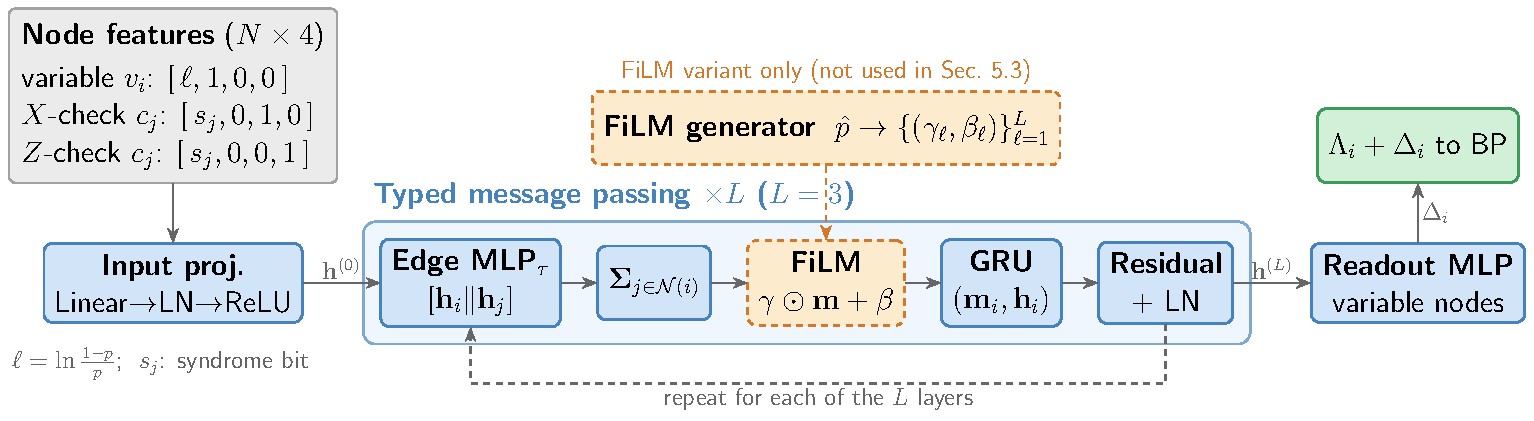
\includegraphics[width=\textwidth]{fig_tannergnn_arch}
\caption{\textsc{TannerGNN} architecture. Variable and check nodes
         exchange typed messages over $L=3$ layers via edge-type-specific
         MLPs; a GRU update with a residual connection and layer
         normalisation follows at each node, and a readout MLP on the
         variable nodes gives the LLR corrections. In the FiLM variant
         (dashed), FiLM modulation scales the aggregated messages at
         each layer; the model of Sec.~\ref{sec:gnn_positive} does not
         use FiLM.}
\label{fig:tannergnn_arch}
\end{figure*}

\begin{remark}[Architectural limitation under biased noise]
The current implementation applies the same scalar $\Delta_i$ to
both $\llr_{z,i}$ and $\llr_{x,i}$, and computes GNN input
features from a single prior LLR $\ell$. Under $\eta = 20$, $\llr_{z,i}$
and $\llr_{x,i}$ differ substantially (factor $\approx 1.9$ in
LLR magnitude at $p=0.04$), so a single correction cannot
simultaneously be optimal for both error types. Separate $Z$- and
$X$-readout heads provide a direct way to remove this coupling and should
be tested under the same biased-noise conditions.
\end{remark}

\subsection{FiLM conditioning}\label{sec:film}

Feature-wise Linear Modulation (FiLM)~\cite{Perez2018FiLM} conditions
each GNN layer on an external context. A small generator network maps
the syndrome-weight estimate
$\phat = \|\synd\|_1 / (m_x + m_z)$ to per-layer affine
parameters $(\gamma^{(\ell)}, \beta^{(\ell)}) = \mathrm{FiLMGen}(\phat)$,
modulating hidden activations as
$\tilde{\bvec{h}}^{(\ell)} = \gamma^{(\ell)} \odot \bvec{h}^{(\ell)} + \beta^{(\ell)}$.
This conditioning pathway is designed to let a single model respond to
global changes in the noise level without retraining. It should not be
confused with spatial calibration: $\phat$ is one scalar shared by the
entire graph and therefore contains no direct per-qubit reliability
information. Section~\ref{sec:invariance} establishes a narrower result:
uniform rescaling of the channel prior cannot change the hard decisions
of the underlying unclipped min-sum BP decoder. That invariance does not,
by itself, imply that a GNN cannot use a global scalar as contextual
information.

\subsection{Neural BP and interleaved pipeline}\label{sec:neuralbp}

Differentiable BP generalises~\eqref{eq:vtc}--\eqref{eq:ctv} with
learnable per-iteration scaling weights $w_\mathrm{ch}^{(t)},
w_\mathrm{vtc}^{(t)}, w_\mathrm{ctv}^{(t)} = \mathrm{softplus}(w_\mathrm{raw}^{(t)})$
(softplus ensures positivity; $w_\mathrm{raw}=0$ at initialisation
gives $w \approx \ln 2 \approx 0.693$, recovering near-standard BP).

\begin{algorithm}[t]
\DontPrintSemicolon
\SetAlgoLined
\caption{Interleaved GNN-BP Decoding}\label{alg:interleaved}
\KwIn{$\synd$, channel LLR $\llr$, noise estimate $\phat$}
\KwOut{Error estimate $\ehat$}
$(\gamma,\beta) \leftarrow \mathrm{FiLMGen}(\phat)$\tcp*{Conditioning}
$\Delta^{(1)} \leftarrow \textsc{TannerGNN}(\llr, \synd, \gamma, \beta)$\;
$\llr' \leftarrow \llr + \Delta^{(1)}$\tcp*{Prior correction}
$\llr_\mathrm{mid} \leftarrow \mathrm{NeuralBP}(\llr', \Hmat, T_1)$\;
$p_i^\mathrm{mid} \leftarrow \sigma(-\llr_{\mathrm{mid},i})\;\forall i$\;
$\Delta^{(2)} \leftarrow \textsc{TannerGNN}(\llr_\mathrm{mid}, p^\mathrm{mid}, \synd, \gamma, \beta)$\;
$\llr'' \leftarrow \llr_\mathrm{mid} + \Delta^{(2)}$\tcp*{Mid correction}
$\llr_\mathrm{final} \leftarrow \mathrm{NeuralBP}(\llr'', \Hmat, T_2)$\;
$\hat{e}_i \leftarrow \mathbbm{1}[\llr_{\mathrm{final},i} < 0]\;\forall i$\;
\Return{$\ehat$}
\end{algorithm}

Algorithm~\ref{alg:interleaved} gives the interleaved pipeline.
The GNN intervenes twice: before BP to correct channel priors, and
after $T_1$ iterations using the intermediate posterior information.
Qubits with $p_i^\mathrm{mid} \approx 0.5$ have low posterior
confidence and can receive a second learned correction. Both correction
stages are trained jointly through the differentiable BP unroll.

\begin{figure*}[t]
\centering
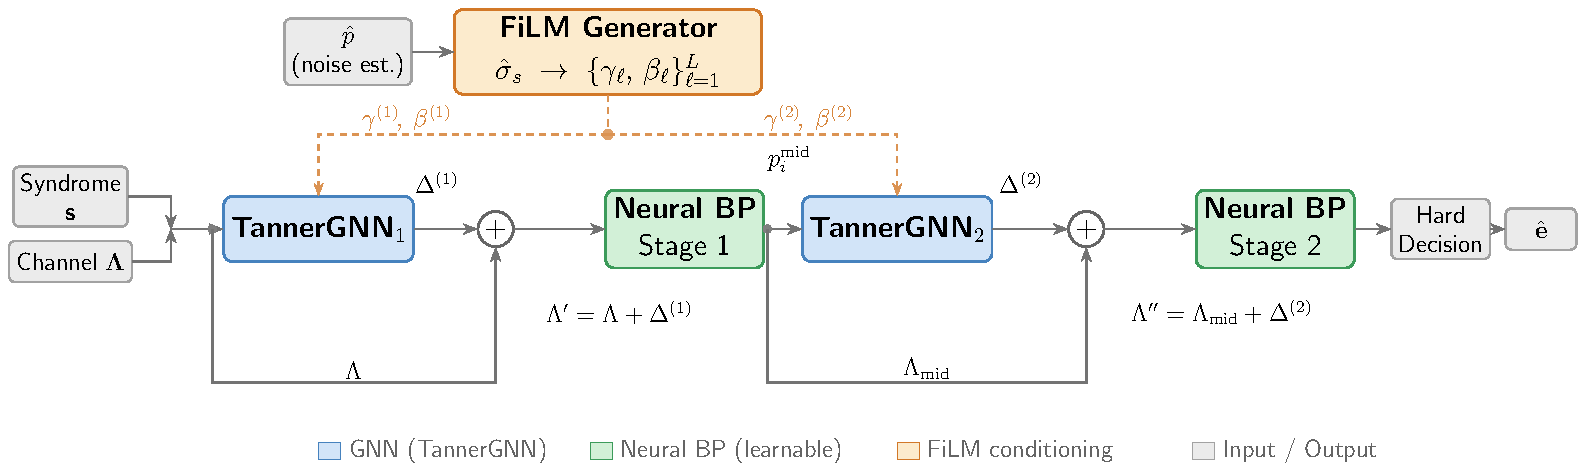
\includegraphics[width=\textwidth]{fig_interleaved_pipeline}
\caption{Interleaved GNN-BP pipeline. The GNN applies two successive
         LLR corrections: one before BP initialisation and one after
         $T_1$ iterations, using the mid-decoding posterior as an
         additional input. Both stages are trained end-to-end through
         the BP unroll.}
\label{fig:interleaved_pipeline}
\end{figure*}

\subsection{Training}\label{sec:training}

\begin{table}[t]
\centering
\footnotesize
\caption{Architecture and training configuration of the
         \textsc{TannerGNN} model of Secs.~\ref{sec:gnn_positive}
         and~\ref{sec:mismatch}.}
\label{tab:hparams}
\setlength{\tabcolsep}{3pt}
\begin{tabular}{@{}ll@{}}
\toprule
\multicolumn{2}{@{}l}{\textit{GNN architecture}} \\
\midrule
Layers $L$ / width $d_h$       & 3 / 32 \\
Edge types                      & 2 ($\Hmat_x$, $\Hmat_z$) \\
Node update                     & GRU, residual, layer norm \\
Node feature dim.               & 4 \\
FiLM / attention                & not used \\
Parameters                      & 39{,}329 \\
\midrule
\multicolumn{2}{@{}l}{\textit{Training}} \\
\midrule
Data                            & \makecell[l]{8{,}000 shots, sinusoidal drift,\\$p\in[0.005,0.045]$} \\
Loss                            & \makecell[l]{focal, $(\alpha,\gamma)=(0.25,2.0)$, on $e_z$;\\no syndrome term} \\
Optimizer                       & \makecell[l]{AdamW, lr $2\times10^{-3}$,\\weight decay $10^{-4}$} \\
Batch size / epochs             & 64 / 20, gradient clipping 1.0 \\
Checkpoint                      & \makecell[l]{fewest failures on\\4{,}000 validation shots} \\
Training seeds                  & 5 \\
BP in training loop             & \makecell[l]{flooding min-sum,\\scaling 0.8, 10 iter.} \\
\midrule
\multicolumn{2}{@{}l}{\textit{Reference BP-OSD baseline}} \\
\midrule
\texttt{bp\_method}             & \texttt{ms} (min-sum) \\
\texttt{ms\_scaling\_factor}    & $0.8$ \\
\texttt{schedule}               & \texttt{serial} (layered) \\
\texttt{max\_iter}              & 100 \\
OSD (where used)                & \texttt{osd\_cs}, order 10 \\
\bottomrule
\end{tabular}
\end{table}

For a shot with prior LLR $\ell=\ln\bigl((1-p)/p\bigr)$ on every qubit,
the GNN outputs a correction $\Delta_j$ for each qubit $j$, giving the
corrected error probability $q_j=\sigma\bigl(-(\ell+\Delta_j)\bigr)$.
The model of Sec.~\ref{sec:gnn_positive} is trained with the focal
loss~\cite{Lin2017Focal} against the true $Z$ error $e_z$,
\begin{equation}
\mathcal{L}=-\frac{1}{Bn}\sum_{b=1}^{B}\sum_{j=1}^{n}
\alpha_{t}\,(1-q_{t})^{\gamma}\log q_{t},
\label{eq:loss}
\end{equation}
where $q_t=q_j$ and $\alpha_t=\alpha$ if $e_{z,j}=1$, and $q_t=1-q_j$
and $\alpha_t=1-\alpha$ otherwise, with $\alpha=0.25$ and $\gamma=2$;
no syndrome-consistency term is used, and the corrected LLRs
$\ell+\Delta_j$ are passed to both CSS components. The training data are
8{,}000 shots from two sinusoidally drifting streams,
$p(t)=p_0+0.015\sin(2\pi t/500)$ with $p_0\in\{0.02,0.03\}$, so the
training rates span $p\in[0.005,0.045]$. The FiLM and interleaved
variants of Secs.~\ref{sec:film}--\ref{sec:neuralbp} are trained on data
regenerated each epoch with $p\sim\mathrm{Uniform}[0.01,0.10]$, and add a
syndrome-consistency term, the binary cross-entropy between the measured
syndrome and $\tfrac12\bigl(1-\prod_{j\in\mathcal N(c)}(1-2q_j)\bigr)$
for each check $c$, with weight $0.1$. Table~\ref{tab:hparams} summarises
the configuration.

% ============================================================
%  IV. EXPERIMENTAL SETUP
% ============================================================
\section{Experimental Setup}\label{sec:setup}

\begin{figure*}[t]
\centering
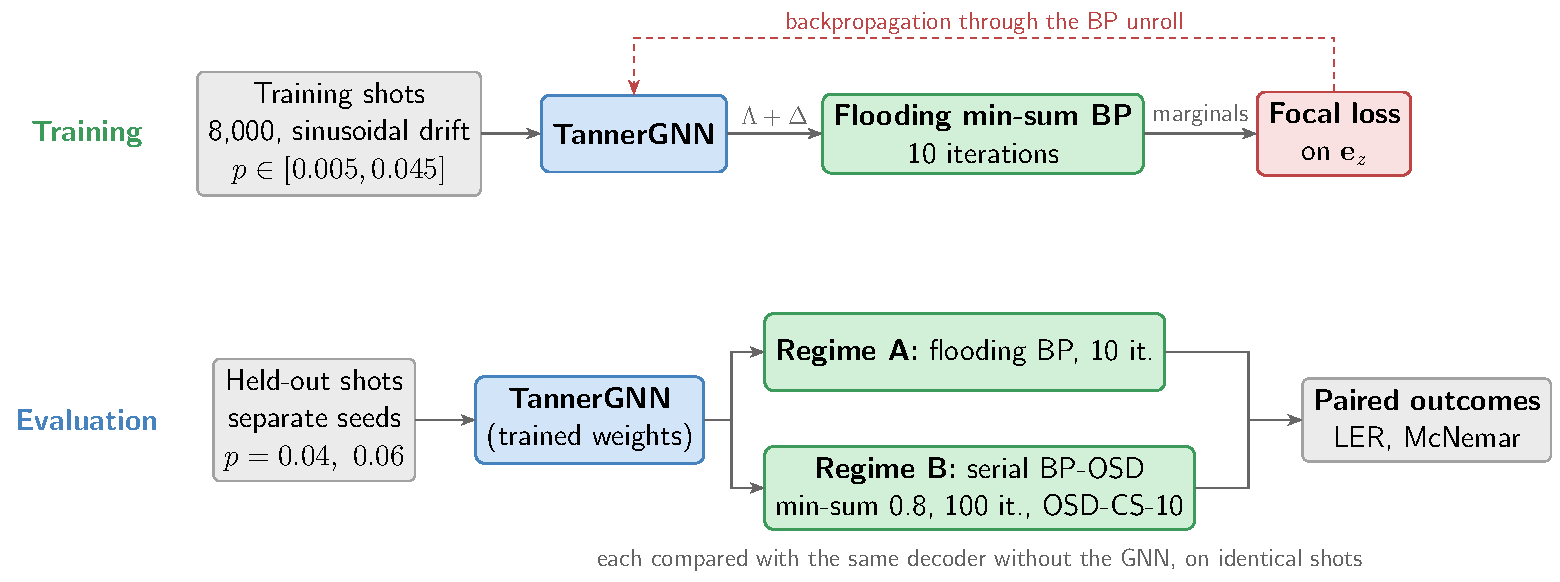
\includegraphics[width=\textwidth]{fig_experimental_pipeline}
\caption{Training and evaluation pipeline of the GNN experiments. The
         GNN is trained through 10-iteration flooding BP and evaluated on
         separately seeded held-out shots in Regime~A (flooding BP) and
         Regime~B (serial BP-OSD); each decoder receives identical
         syndrome batches to enable McNemar paired testing.}
\label{fig:experimental_pipeline}
\end{figure*}

\subsection{Evaluation regimes}\label{sec:regimes}

Two distinct evaluation regimes are used throughout this paper,
and the distinction is central to interpreting the results:

\textbf{Regime A (training-aligned baseline):} The GNN is evaluated
against flooding BP, the base decoder used during training. This
comparison isolates the gain relative to the decoder represented in the
training computation graph.

\textbf{Regime B (stronger classical baseline):} The same learned
correction is evaluated with the serial-schedule min-sum BP-OSD reference
configuration. This tests whether the correction also improves the
stronger classical decoder considered here; Sec.~\ref{sec:mismatch}
shows that it does not in the tested regime.

Unless otherwise stated, all experiments use $Z$-biased noise with
$\eta = 20$.

\subsection{Statistical protocol}\label{sec:metrics}

\paragraph{Logical failure.} For each shot let $\hat{e}_z$ and
$\hat{e}_x$ be the decoder's hard decisions and $r_z=e_z\oplus\hat{e}_z$,
$r_x=e_x\oplus\hat{e}_x$ the residual errors. A shot is a logical failure
if (i) the estimate does not reproduce the measured syndrome,
$\Hmat_x\hat{e}_z\neq s_x$ or $\Hmat_z\hat{e}_x\neq s_z$, or (ii) the
syndrome is reproduced but the residual acts nontrivially on the code
space, $\mathbf{L}_x r_z\neq\mathbf{0}$ or $\mathbf{L}_z r_x\neq\mathbf{0}$
over $\F_2$, where the rows of $\mathbf{L}_x$ ($\mathbf{L}_z$) span the
$k=12$ independent logical operators that detect $Z$ ($X$) errors.
Condition (i) is needed because a syndrome-inconsistent residual is not a
logical operator, so its parity against fixed logical representatives is
not meaningful; non-converged BP outputs therefore always count as
failures. The $X$ and $Z$ components are combined by logical OR, so the
reported LER is the probability that at least one of the 12 logical
qubits suffers a logical error of any Pauli type in a shot. At circuit
level the same rule is applied to the detector error model: a shot fails
if the decoded fault set does not reproduce the detection events, or if
it does and predicts the wrong observable flips.

For absolute LER comparisons we treat operating points with fewer than
100 observed logical-error events as preliminary; this is a reporting
heuristic rather than a formal power calculation. Decoder pairs are
evaluated on \emph{identical} syndrome samples, enabling paired
McNemar tests~\cite{McNemar1947}. We report Wilson score 95\% confidence
intervals for LER estimates.

Training, validation and test data are drawn with distinct random
seeds, so no evaluation shot shares a random stream with a training
shot, and learned-decoder results are reported over five training seeds
(initialisation and minibatch order). All training and evaluation used
CPU only; no GPU was available for this work. One training epoch of the
39k-parameter model of Sec.~\ref{sec:gnn_positive} takes about 16\,s.

% ============================================================
%  V. RESULTS
% ============================================================
\section{Results}\label{sec:results}

\subsection{Decoder configuration sensitivity}\label{sec:baseline}

Before presenting the GNN results, we quantify the sensitivity of the
classical baseline to decoder configuration. This sensitivity sets the
scale against which the learned-decoder results must be interpreted.

\begin{table*}[t]
\centering
\caption{Effect of BP-OSD configuration on $\code{288}{12}{18}$,
         $p=0.04$, $\eta=20$, 100{,}000 identical shots, priors $p_z$ and
         $p_x$ of Eq.~\eqref{eq:bias}. 95\% Wilson intervals in brackets.}
\label{tab:smoking_gun}
\begin{tabular}{@{}llllcc@{}}
\toprule
Config & Schedule & Method & Iter & LER & Errors \\
\midrule
Original BP     & parallel & prod-sum & 30  & 0.0569 [0.0555,0.0583] & 5{,}689 \\
Reference BP    & serial   & ms(0.8)  & 100 & 0.0017 [0.0015,0.0020] &    174 \\
Original BP-OSD & parallel & prod-sum & 30  & 0.0398 [0.0386,0.0411] & 3{,}983 \\
Ref.\ BP-OSD    & serial   & ms(0.8)  & 100 & 0.00034 [0.00024,0.00048] &   34 \\
\bottomrule
\end{tabular}
\end{table*}

Table~\ref{tab:smoking_gun} illustrates how strongly decoder
configuration changes the finite-length result. The original parallel
product-sum BP-OSD configuration reduces LER from $0.0569$ to $0.0398$
relative to the corresponding plain BP, but remains far worse than the
serial min-sum configurations. The reference serial min-sum BP-OSD
records 34 logical errors in $10^5$ shots, so its value is preliminary
by the criterion of Sec.~\ref{sec:metrics}.

A separate $N=100{,}000$-shot experiment (Fig.~\ref{fig:baseline_decomp})
changes one factor at a time. The flooding comparator is min-sum BP with
scaling factor $0.8$, at most 100 iterations, stopping at the first
iteration whose hard decision satisfies the syndrome, with a parallel
(flooding) schedule; the second decoder is identical except for the
serial schedule; the third adds OSD-CS-10. The LER falls from
$1.28\times10^{-2}$ to $1.45\times10^{-3}$ ($8.8\times$, paired
$n_{10}/n_{01}=1138/3$) and then to $2.7\times10^{-4}$ ($5.4\times$,
$118/0$), about $47\times$ overall.

\begin{figure}[t]
\centering
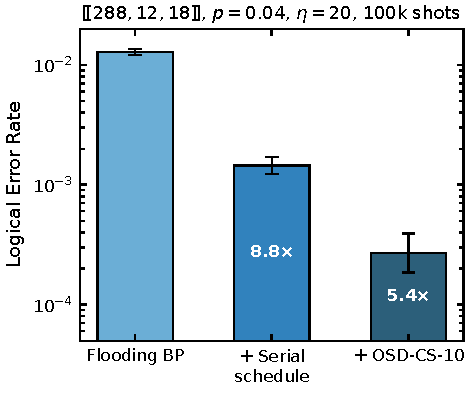
\includegraphics[width=\columnwidth]{fig_F1_baseline_decomp}
\caption{Baseline decomposition on $\code{288}{12}{18}$, $p=0.04$,
         $\eta=20$, 100k identical shots. Min-sum BP (scaling 0.8, at most
         100 iterations) with flooding and then serial schedule, then
         serial BP-OSD-CS-10. Wilson 95\% CI error bars; labels give the
         factor gained at each step.}
\label{fig:baseline_decomp}
\end{figure}

These data do not identify a universally optimal configuration. They do
show that schedule, update rule, iteration budget, and post-processing
can dominate the measured finite-length LER. Learned-decoder comparisons
must therefore specify and control these parameters.

\subsection{Uniform-prior scaling invariance of min-sum BP}\label{sec:invariance}

\begin{proposition}[Uniform positive-scaling invariance]\label{prop:invariance}
Consider separate-CSS min-sum BP with no message clipping or offset. If
all channel LLRs in one CSS component are multiplied by the same factor
$a>0$, then every BP message and posterior LLR is multiplied by $a$ at
every iteration. Consequently, all hard decisions are unchanged.
\end{proposition}

\begin{proof}
At initialization, each variable-to-check message is proportional to the
corresponding channel LLR and therefore scales by $a$. Assume all
variable-to-check messages at iteration $t$ have scaled by $a$. The
syndrome factor $(-1)^{s_j}$ in Eq.~\eqref{eq:ctv} is unchanged, the sign
of every message is unchanged because $a>0$, and
$\min_i a|x_i|=a\min_i|x_i|$. Hence every check-to-variable message also
scales by $a$. Equation~\eqref{eq:vtc} then shows that the next
variable-to-check messages scale by $a$. Induction establishes the claim
for all iterations and for the final posterior LLRs.
\end{proof}

For a uniform channel prior, replacing a common positive LLR $\Lambda$
by another positive value $\Lambda'$ is equivalent to the scaling
$a=\Lambda'/\Lambda$. The proposition explains why changing only the assumed uniform physical
error rate cannot change hard decisions of ideal min-sum BP. Clipping, offsets, damping rules that depend on
magnitude, non-uniform priors, or sum-product updates can break the exact
scaling argument.

We checked the proposition on 2{,}000 shots each. With unclipped
min-sum BP (serial or flooding, 100 iterations), changing the assumed
uniform rate from $p=0.015$ to $p=0.0286$ on $\code{288}{12}{18}$, or from
$p=0.04$ to $p=0.02$ on $\code{72}{12}{6}$, leaves every hard decision
unchanged (2{,}000/2{,}000). Two cases fall outside the proposition, and
the invariance fails there: our PyTorch min-sum implementation clamps
messages to $\pm20$ and changes 18 of 2{,}000 decisions on
$\code{288}{12}{18}$, and sum-product BP changes 25--43 of 2{,}000.

\begin{remark}[What the proposition does and does not imply]
The result applies to the BP pathway when adaptivity enters only by
changing a uniform channel-prior magnitude. It does \emph{not} establish
that a global conditioning scalar is information-theoretically useless
to a GNN: a learned model could combine a global noise estimate with
local syndrome structure and change its nonlinear decision rule. The experiments below test a narrower hypothesis: spatially resolved
per-qubit calibration can change the relative reliabilities seen by the
decoder, whereas a single graph-wide scalar cannot provide that spatial
information.
\end{remark}

\subsection{GNN improvement over flooding BP}\label{sec:gnn_positive}

We evaluated the GNN against flooding BP---the decoder it was
trained against---on separately seeded held-out syndromes: 4{,}000
validation shots at $p=0.04$ select the checkpoint over 20 epochs, and
test sets of 20{,}000 shots at $p=0.04$ (inside the training range) and
10{,}000 shots at $p=0.06$ (outside it) are each scored once on that
checkpoint. Training is repeated with five seeds.

\begin{table}[t]
\centering
\caption{GNN-BP vs.\ flooding BP on $\code{72}{12}{6}$, $\eta=20$,
         20{,}000 ($p=0.04$) and 10{,}000 ($p=0.06$) held-out test
         syndromes, five training seeds (mean $\pm$ s.d.). $n_{10}$
         ($n_{01}$): shots only BP (only GNN-BP) fails. BP is flooding
         min-sum.}
\label{tab:gnn_flooding}
\footnotesize
\setlength{\tabcolsep}{3.5pt}
\begin{tabular}{@{}lcc@{}}
\toprule
 & $p=0.04$ & $p=0.06$ \\
\midrule
BP, 10 iter.                 & 0.1077 & 0.2867 \\
GNN-BP, 10 iter.             & $0.0942\pm0.0006$ & $0.2564\pm0.0019$ \\
\quad relative reduction     & $12.5\%\pm0.6\%$ & $10.6\%\pm0.7\%$ \\
\quad $n_{10}$ / $n_{01}$    & 313--370 / 64--95 & 343--394 / 66--80 \\
BP, 100 iter.                & 0.0863 & 0.2403 \\
Serial BP-OSD                & 0.0707 & 0.2138 \\
\bottomrule
\end{tabular}
\end{table}

Table~\ref{tab:gnn_flooding} gives the primary learned-decoder result.
Over five training seeds, GNN-BP reduces LER relative to flooding BP by
$12.5\%\pm0.6\%$ at $p=0.04$ and by $10.6\%\pm0.7\%$ at $p=0.06$, outside
the training range (McNemar $p<10^{-36}$ for every seed). The gain comes
mostly from convergence: shots on which BP does not reproduce the
syndrome fall from 1{,}740 to 838--975 of 20{,}000. Flooding BP with 100
iterations and serial BP-OSD both remain better than GNN-BP. A gradient audit found non-zero
signal through the network (input-to-readout gradient ratio $0.63$--$2.19$
over the five seeds) and non-trivial LLR corrections (mean
$|\Delta_i|=0.54$--$1.01$).

A fixed-dataset capacity test provides an additional diagnostic: a GNN
trained on 1{,}000 fixed syndromes for 50 epochs reduced the failure
count on those same syndromes from 105 to 93 ($11\%$; McNemar
$p=0.0095$, $n_{10}=15$, $n_{01}=3$). This experiment tests the ability of
the architecture and optimizer to fit the supplied examples; it is not a
generalization result. The interleaved architecture of
Sec.~\ref{sec:neuralbp} is not evaluated in this work.

\subsection{Training/evaluation baseline mismatch}\label{sec:mismatch}

Although the GNN improves flooding BP, the same correction does not
improve the serial min-sum BP-OSD reference configuration. Note that Tables~\ref{tab:gnn_flooding}
and~\ref{tab:gnn_null} report different evaluation regimes
(Regime~A and Regime~B of Sec.~\ref{sec:regimes}) on different
syndrome sets, and their LER values are not directly comparable.

\begin{table}[t]
\centering
\caption{GNN-BP vs.\ serial BP-OSD on $\code{72}{12}{6}$, $\eta=20$,
         20{,}000 identical shots per $p$, five training seeds. Last
         column: seeds for which GNN+OSD is significantly worse
         (McNemar $p<0.05$).}
\label{tab:gnn_null}
\footnotesize
\begin{tabular}{@{}lccc@{}}
\toprule
$p$ & Serial BP-OSD & GNN+OSD & Seeds worse \\
\midrule
0.020 & 0.0093 & 0.0095--0.0102 & 1/5 \\
0.030 & 0.0297 & 0.0306--0.0317 & 5/5 \\
0.040 & 0.0676 & 0.0688--0.0709 & 4/5 \\
0.050 & 0.1354 & 0.1384--0.1418 & 5/5 \\
\bottomrule
\end{tabular}
\end{table}

\begin{figure}[t]
\centering
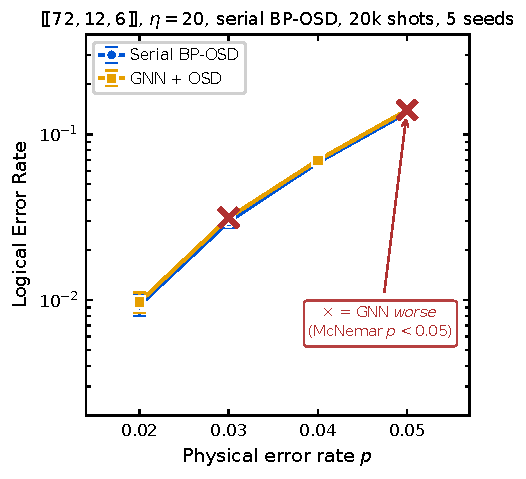
\includegraphics[width=\columnwidth]{fig_F4_phase4_ler}
\caption{GNN+OSD vs.\ serial BP-OSD LER on $\code{72}{12}{6}$,
         $\eta=20$, 20{,}000 shots per point; GNN+OSD is the mean over
         five training seeds. Red $\times$ marks operating points where
         every seed is statistically worse (McNemar $p<0.05$).
         Wilson 95\% CI error bars.}
\label{fig:gnn_null_curve}
\end{figure}

Table~\ref{tab:gnn_null} and Fig.~\ref{fig:gnn_null_curve} show that
the GNN-corrected decoder never improves on serial BP-OSD: at $p=0.02$
one seed of five is significantly worse, and from $p=0.03$ on 14 of 15
seed--error-rate pairs are significantly \emph{worse}. The same checkpoints improve flooding BP, so these
data show that the learned correction does not transfer unchanged to the
stronger decoder.

The GNN was optimized through a
10-iteration flooding-BP computation graph and is then inserted ahead of
a decoder with a different schedule, iteration budget, and OSD
post-processing.

\begin{table}[t]
\centering
\caption{Paired failure sets on $\code{72}{12}{6}$, $p=0.04$, $\eta=20$,
         20{,}000 identical held-out shots. BP: 10-iteration flooding BP.
         GNN rows give the range over five training seeds. ``Non-conv.'':
         the estimate does not reproduce the syndrome.}
\label{tab:failure_sets}
\footnotesize
\setlength{\tabcolsep}{3pt}
\begin{tabular}{@{}lcc@{}}
\toprule
Decoder & Failures & Non-conv. \\
\midrule
BP, 10 iter.            & 2{,}155 & 1{,}740 \\
BP, 100 iter.           & 1{,}727 & 700 \\
Serial BP-OSD           & 1{,}414 & 0 \\
GNN + BP, 10 iter.      & 1{,}874--1{,}906 & 838--975 \\
GNN + BP-OSD            & 1{,}439--1{,}451 & 0 \\
\midrule
\multicolumn{3}{@{}l}{\textit{Overlaps}} \\
\makecell[l]{BP-OSD failures\\also failed by BP} & \multicolumn{2}{c}{1{,}319 / 1{,}414 (93\%)} \\
\makecell[l]{BP-100 failures\\also failed by BP} & \multicolumn{2}{c}{1{,}727 / 1{,}727 (100\%)} \\
Shots GNN fixes for BP            & \multicolumn{2}{c}{313--370} \\
\quad of which BP did not converge & \multicolumn{2}{c}{91--93\%} \\
\quad of which BP-OSD also fails   & \multicolumn{2}{c}{31--36\%} \\
\makecell[l]{BP-OSD failures also\\failed by GNN+BP} & \multicolumn{2}{c}{87--88\%} \\
\makecell[l]{GNN+BP-OSD vs.\ BP-OSD:\\newly failed / rescued} & \multicolumn{2}{c}{237--282 / 206--254} \\
\bottomrule
\end{tabular}
\end{table}

A paired failure-set analysis (Table~\ref{tab:failure_sets}) shows that
the two decoders do not fail on disjoint sets: every shot that
100-iteration BP fails is also failed by 10-iteration BP, and 93\% of
BP-OSD's failures are BP failures. What separates them is mainly
convergence: 81\% of BP failures are shots on which BP does not reach a
syndrome-consistent estimate, whereas BP-OSD always returns one. Of the
313--370 shots the GNN fixes for BP, 91--93\% are non-converged BP shots
and only 31--36\% are shots that BP-OSD fails, so the GNN's gains lie
mostly where BP-OSD already succeeds. When the same corrections are
passed to BP-OSD they reshuffle its failures (237--282 newly failed vs.\
206--254 rescued shots), almost entirely among shots on which BP itself
fails. The same pattern holds at $p=0.06$, where 96\% of BP-OSD failures
are BP failures. Training directly against the target decoder, or against a
differentiable surrogate of its post-processing stage, remains the
appropriate test of whether learned augmentation can improve BP-OSD.

\subsection{Per-qubit calibration gap}\label{sec:oraclegap}

Under spatially non-uniform per-qubit noise, each data qubit has rate
$p_i=p\,e^{\sigma z_i-\sigma^2/2}$ with $z_i\sim\mathcal N(0,1)$ drawn
fresh every shot (capped at 0.5), so the mean rate is $p$ for every
$\sigma$. A decoder knowing the true per-qubit rates (serial min-sum
BP-OSD-CS-10 with the true $p_i$ as priors) substantially outperforms a
decoder using the uniform mean prior $p$.

\begin{figure}[t]
\centering
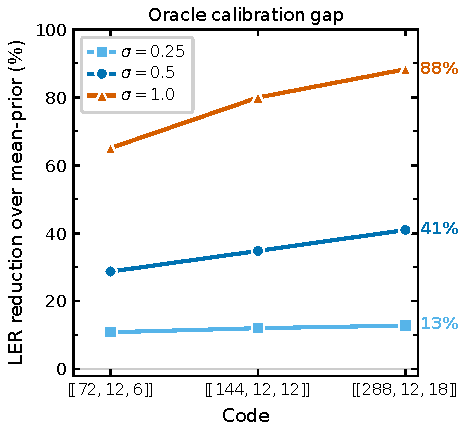
\includegraphics[width=\columnwidth]{fig_F2_oracle_vs_distance}
\caption{Oracle calibration gap (percentage LER reduction from
         per-qubit vs.\ mean-prior BP-OSD), 50k identical shots per
         point.
         Operating points: $p=0.04$, $0.06$, $0.07$ respectively;
         cross-code comparisons are partially confounded by the
         differing operating points.}
\label{fig:oracle_gap}
\end{figure}

\begin{table*}[t]
\centering
\caption{Oracle gap: percentage LER reduction from per-qubit
         over mean-prior BP-OSD, 50{,}000 identical shots per cell, at
         $p=0.04$, $0.06$, $0.07$ for the three codes. All McNemar
         $p<10^{-20}$. Parenthetical counts are mean-prior error events.}
\label{tab:oracle}
\begin{tabular}{@{}lccc@{}}
\toprule
Code ($d$) & $\sigma=0.25$ & $\sigma=0.5$ & $\sigma=1.0$ \\
\midrule
$\code{72}{12}{6}$   (6)  & $+11\%$ (3508) & $+29\%$ (3432) & $+65\%$ (3438) \\
$\code{144}{12}{12}$ (12) & $+12\%$ (3165) & $+35\%$ (3203) & $+80\%$ (2936) \\
$\code{288}{12}{18}$ (18) & $+13\%$ (3338) & $+41\%$ (3307) & $+88\%$ (2786) \\
\bottomrule
\end{tabular}
\end{table*}

Table~\ref{tab:oracle} and Fig.~\ref{fig:oracle_gap} show a clear
increase with noise contrast $\sigma$ for each tested code. The reported
percentage reduction is also larger for the larger-code rows, reaching
$88\%$ on $\code{288}{12}{18}$ at $\sigma=1.0$; however, the physical
error rate is changed across codes ($p=0.04$, $0.06$, and $0.07$).
Consequently, these data do not isolate code distance as the cause of
the cross-code trend.

This experiment isolates the value of synthetic per-qubit rate side
information; it does not require machine learning. We use the true-rate
decoder as an \emph{oracle reference}, not as a formal upper bound on all
possible decoders. The comparison quantifies how much the tested BP-OSD
implementation can benefit when the realized per-qubit rates are
revealed. The gap is \emph{not}
recoverable from a single syndrome shot under i.i.d.\ per-qubit
noise: with a fresh field redrawn every shot, the uniform mean
prior is Bayes-optimal within the class of estimators that observe
only the syndrome, so no syndrome-conditioned GNN can do better
than the mean prior in this regime.

\subsection{Drift adaptation}\label{sec:drift}

Under persistent OU drift ($\sigma=1.0$, $W=32$-round window,
$\code{72}{12}{6}$, $p=0.04$, 6{,}000 shots), the GNN beats
stale calibration only at the highest tested drift volatility.

\begin{table*}[t]
\centering
\caption{LER under per-qubit OU drift by volatility (vol).
         ``Empir'': non-learned per-qubit frequency estimator.}
\label{tab:drift}
\begin{tabular}{@{}lccccl@{}}
\toprule
vol & Oracle & Stale & Empir & GNN & Verdict \\
\midrule
0.00 & 0.033 & 0.033 & 0.057 & 0.064 & GNN worse, $p=5\!\times\!10^{-36}$ \\
0.10 & 0.031 & 0.038 & 0.057 & 0.067 & GNN worse, $p=8\!\times\!10^{-30}$ \\
0.35 & 0.005 & 0.027 & 0.038 & 0.050 & GNN worse, $p=5\!\times\!10^{-19}$ \\
0.50 & 0.004 & 0.052 & 0.035 & \textbf{0.044} & GNN beats stale, $p=0.005$ \\
\bottomrule
\end{tabular}
\end{table*}

\begin{figure}[t]
\centering
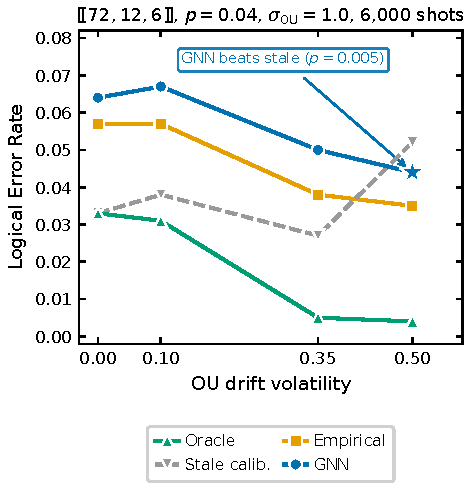
\includegraphics[width=\columnwidth]{fig_F3_drift_adaptation}
\caption{LER vs.\ OU drift volatility for four decoder configurations
         on $\code{72}{12}{6}$, $p=0.04$, $\sigma_\mathrm{OU}=1.0$, 6{,}000 shots.
         Star marks the single operating point (vol$=0.5$) where GNN
         beats stale calibration ($p=0.005$); GNN is beaten by the
         empirical frequency estimator at every volatility level.}
\label{fig:drift_curve}
\end{figure}

Table~\ref{tab:drift} and Fig.~\ref{fig:drift_curve} show that the GNN beats stale calibration
at vol$=0.5$ ($p=0.005$, 158 vs.\ 111 discordant pairs), but
is beaten by the non-learned empirical frequency estimator at
every volatility level (GNN vs.\ empir: $p = 2.7\times10^{-8}$
at vol$=0.5$, GNN worse). Under independent per-qubit drift,
direct per-qubit syndrome frequency counting captures most of
the available signal, leaving little room for a learned estimator.
Whether spatial correlation structure between qubits would shift
this result is an open question.

\subsection{Circuit-level evaluation}\label{sec:circuit}

\paragraph{Circuit and noise model.} We simulate a $Z$-basis memory
experiment on $\code{72}{12}{6}$ with 6 rounds of syndrome extraction
(72 data qubits, 36 $X$-check and 36 $Z$-check ancillas). Data qubits are
prepared in $\ket{0}$; each round measures all $X$-checks and then all
$Z$-checks with dedicated ancillas, using CNOT layers from a greedy
conflict-free schedule; the data qubits are finally measured in the $Z$
basis. Detectors are (i) the 36 $Z$-checks of round 1, which are
deterministic for the prepared state, (ii) the XOR of consecutive
measurements of every check in rounds 2--6, and (iii) the XOR of the last
$Z$-check outcome with the parity of the measured data qubits in its
support, giving 432 detectors and 12 logical observables. Noise is a
biased single-qubit Pauli channel with $p_X=p/(\eta+1)$,
$p_Z=p\,\eta/(\eta+1)$, $p_Y=0$, $\eta=20$, applied to every qubit after
each one- and two-qubit gate and to every idle qubit at each time step;
measurements and resets flip with probability $p$. Under spatially
non-uniform noise each qubit $q$ (data and ancilla) has rate
$p_q=p\,e^{\sigma z_q-\sigma^2/2}$, $z_q\sim\mathcal N(0,1)$, $\sigma=1$,
on all of its fault locations, so the mean rate is $p$ as in
Sec.~\ref{sec:oraclegap}.

\paragraph{Decoders.} We decode the detector error model (4{,}068 fault
mechanisms) with serial min-sum BP-OSD (scaling 0.8, 100 iterations,
OSD-CS order 10), as in Table~\ref{tab:hparams}. The mean-prior decoder
uses the uniform rate $p$; the oracle uses the true $p_q$. We draw
20 rate profiles at $p\le0.003$ and 40 at
$p=0.01$, with 500 shots per profile. Failures follow
Sec.~\ref{sec:metrics}.

\begin{table}[t]
\centering
\caption{Circuit-level oracle gap on $\code{72}{12}{6}$ (6 rounds,
         $\eta=20$, $\sigma=1$). $n_{10}$ ($n_{01}$): shots only the
         mean-prior decoder (only the oracle) fails. Zero failures in
         $10^4$ shots means LER $<3.8\times10^{-4}$ (95\% upper bound).}
\label{tab:circuit}
\footnotesize
\setlength{\tabcolsep}{4pt}
\begin{tabular}{@{}lccccc@{}}
\toprule
$p$ & Shots & Mean prior & Oracle & $n_{10}/n_{01}$ & $p_\mathrm{McN}$ \\
\midrule
0.001 & 10{,}000 & 0 & 0 & 0/0 & --- \\
0.003 & 10{,}000 & 0 & 0 & 0/0 & --- \\
0.01  & 20{,}000 & $1.35\%$ & $0.60\%$ & 177/28 & $5\!\times\!10^{-25}$ \\
\bottomrule
\end{tabular}
\end{table}

\begin{figure}[t]
\centering
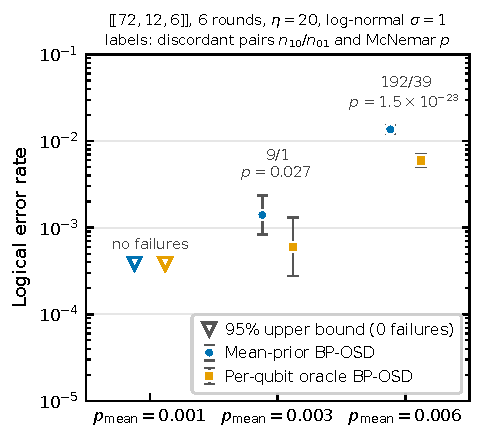
\includegraphics[width=\columnwidth]{fig_F6_circuit_oracle}
\caption{Circuit-level oracle gap on $\code{72}{12}{6}$, 6 rounds,
         $\eta=20$, $\sigma=1$. Points: LER with 95\% Wilson intervals;
         open triangles: 95\% upper bound when no failures were
         observed. Labels: discordant pairs and McNemar $p$.}
\label{fig:circuit_null}
\end{figure}

Knowing the per-qubit rates also helps at circuit level
(Table~\ref{tab:circuit}, Fig.~\ref{fig:circuit_null}). At $p=0.01$ the
oracle reduces the logical error rate from $1.35\%$ to $0.60\%$ ($55\%$;
McNemar $p=4.8\times10^{-25}$), and it is better on 38 of 40 independent
rate profiles (sign test $p=1.5\times10^{-9}$), so the result is not
driven by a few extreme profiles. At $p=0.001$ and $p=0.003$ neither
decoder fails in $10^4$ shots, so these operating points cannot resolve a
gap. The circuit-level gap is somewhat smaller than the code-capacity gap
on the same code ($65\%$ at $\sigma=1$, Table~\ref{tab:oracle}), at a
different operating point, but it does not vanish.

% ============================================================
%  VI. DISCUSSION
% ============================================================
\section{Discussion}\label{sec:discussion}

\subsection{The GNN's role and its limits}

\textsc{TannerGNN} reduces the LER of the flooding BP decoder used in
its training loop by $12.5\%\pm0.6\%$ over five training seeds, and
gradient diagnostics show that the network produces non-trivial
corrections. The gain comes mainly from helping BP converge, and
100-iteration BP and serial BP-OSD remain stronger than the corrected
decoder.

The Regime-B result is also informative: the learned correction does
not transfer automatically to serial BP-OSD. This is consistent with the
training/evaluation mismatch: the failure sets of BP and BP-OSD are
nested, and the GNN's repairs fall mostly on shots BP-OSD already
decodes (Table~\ref{tab:failure_sets}).
Training against BP-OSD directly is complicated by the non-differentiable
OSD stage; differentiable surrogates, distillation, or training on the
residual failures of the target decoder are possible alternatives.

\subsection{Benchmark design implications}

The baseline experiments identify two reporting requirements for learned
QLDPC decoders. First, BP-OSD schedule, update rule, iteration count, and
OSD configuration must be stated explicitly because they can change LER
by more than two orders of magnitude on the same code. Table~\ref{tab:hparams}
records these settings for the present study.

Second, the training and evaluation decoders must be distinguished. An
LLR correction learned through flooding BP need not remain beneficial
when the schedule, iteration count, and OSD stage are changed. Comparisons
across such decoder configurations should identify the mismatch rather
than treating all BP-based baselines as equivalent.

\subsection{Comparison with prior work}\label{sec:priorwork}

Astra~\cite{Maan2025MLBP} uses a learned Tanner-graph message-passing
decoder and reports BB-code performance competitive with, and in several
settings better than, BP-OSD under code-capacity depolarizing noise. This
places our $12.5\%$ flooding-BP gain in context: improvement over plain BP
is not, by itself, the main novelty. Our contribution is instead the
controlled comparison showing how that gain changes when the baseline
and side information are strengthened.

Gong et al.~\cite{Gong2024GNN} interleave differentiable BP stages with
GNN corrections on the same sparse graph and show error-floor
improvements over several post-processing approaches. Our interleaved
variant follows the same broad design principle, but its decoding
performance is not evaluated here, so we do not claim a competitive
result for that architecture.

Recent circuit-level work on BB codes also reports neural decoders that
can outperform BP-OSD on the $\code{72}{12}{6}$ code while retaining a
runtime advantage, although scaling to $\code{144}{12}{12}$ remains more
challenging~\cite{Blue2026MLBB}. This comparison reinforces the need to evaluate learned decoders against
a fully specified competitive non-learned baseline, not only against
flooding BP.

Stein et al.~\cite{Stein2026FiLM} condition a neural QEC decoder on
spatially resolved hardware calibration data using FiLM and evaluate on
IBM repetition-code experiments. Their conditioning signal is per-qubit
and calibration-derived, unlike the single scalar $\phat$ used in our
initial model. This distinction is consistent with the oracle experiments
of Sec.~\ref{sec:oraclegap}, which motivate spatial rather than purely
global conditioning.
\subsection{Towards spatially-resolved conditioning}\label{sec:srcf}

The oracle-gap experiment (Sec.~\ref{sec:oraclegap}) shows that
per-qubit rate side information can materially improve the tested
BP-OSD decoder. Because operating point and code size co-vary, the
current data do not establish how this value scales with distance.
Proposition~\ref{prop:invariance} also shows that a uniform rescaling
of the min-sum BP prior cannot reproduce the effect of spatially varying
reliabilities. These results motivate testing spatially resolved FiLM
(SRCF), in which per-qubit parameters $(\gamma_i, \beta_i)$ are
conditioned on persistent hardware calibration data rather than on a
single graph-wide scalar. Such a decoder should be compared with the
non-learned frequency estimator of Sec.~\ref{sec:drift} and evaluated
in a circuit-level setting where the calibration signal remains
identifiable. Neither condition has been established in the present
experiments.

\subsection{Limitations}\label{sec:limitations}

\begin{enumerate}[leftmargin=*,topsep=3pt,itemsep=2pt,
                  label=(\roman*)]
\item All GNN variants were trained against 10-iteration
      flooding BP. No variant was trained against serial BP-OSD,
      which is the competitive classical baseline. Whether GNN
      augmentation of serial BP-OSD yields gains is untested.
\item GNN checkpoints exist only for $\code{72}{12}{6}$; the
      larger codes were not trained due to CPU-only compute
      constraints. The null result in Regime B should not be
      extrapolated to the larger codes.
\item The interleaved and FiLM architectures are described but their
      decoding performance is not evaluated.
\item The single per-qubit correction $\Delta_i$ is applied to
      both $\llr_{z,i}$ and $\llr_{x,i}$, which is suboptimal
      under $\eta = 20$ biased noise; separate $Z$/$X$ readout
      heads are the recommended fix.
\item Code-capacity noise omits measurement errors, leakage,
      and correlated faults present in real circuits.
\end{enumerate}

% ============================================================
%  VII. CONCLUSION
% ============================================================
\section{Conclusion}\label{sec:conclusion}

On $\code{72}{12}{6}$, a Tanner-graph GNN trained through
10-iteration flooding BP reduces the held-out LER of that decoder by
$12.5\%\pm0.6\%$ at $p=0.04$ and $\eta=20$ over five training seeds. The
same learned correction does not improve the serial min-sum BP-OSD
reference decoder and is significantly worse from $p=0.03$ on; the shots
it repairs are largely ones BP-OSD already decodes. The demonstrated gain is therefore specific
to the training-aligned flooding-BP baseline; the present experiments do
not establish an improvement over competitive BB decoding more generally.

The baseline experiments show that BP schedule, update rule, iteration
budget, and OSD configuration can change finite-length LER by orders of
magnitude. These parameters must be treated as part of the decoder
specification when learned and non-learned methods are compared. We also
proved that uniform positive rescaling of the channel LLRs leaves the
hard decisions of ideal min-sum BP unchanged. A global prior magnitude
alone therefore cannot provide spatial adaptation to heterogeneous qubit
reliabilities, although a nonlinear learned model may still use a global
noise estimate as context.

The synthetic oracle experiments identify per-qubit calibration as the
more informative adaptive signal in the tested setting: revealing the
true per-qubit rates substantially improves BP-OSD under heterogeneous
noise, and under circuit-level noise it reduces BP-OSD's LER by $55\%$ at
$p=0.01$. The current cross-code experiments do not
isolate how this gain scales with distance. A direct next test is to condition a
learned decoder on persistent spatial calibration data and compare it
against a fully specified serial BP-OSD baseline and the non-learned
frequency estimator, using multiple training seeds and a noise model that
preserves temporal calibration structure.
\section*{Acknowledgments}

The authors thank the STAR Lab program at the University of Arizona
for facilitating this research and providing computational resources.

\section*{Data and code availability}

Source code, trained checkpoints, datasets and the analysis scripts
behind every table and figure except the drift experiment
(Sec.~\ref{sec:drift}) are available at
\url{https://github.com/kondshk/adaptive_gnn}. Code-capacity data are
sampled directly with NumPy; circuit-level data are generated with
Stim~\cite{Gidney2021Stim}.

\setlength{\bibsep}{1pt plus 0.3ex}
\bibliographystyle{quantum}
\bibliography{references}

\end{document}
